\chapter{Fundamentals}
\label{ch:fundamentals}
\section{Virtualisation}
Chapter \ref{ch:fundamentals/virtualisation/axioms} introduces the fundamental axioms that define 
virtualisation - noninterference, isolation and performance. 
Chapter \ref{ch:fundamentals/virtualisation/hardware-virtualisation} presents hardware virtualisation 
as a concept, discusses the mechanisms it uses to satisfy the axioms, and highlights the trade-offs
intrinsic to its design. 
Chapter \ref{ch:fundamentals/virtualisation/os-virtualisation} describes a more coarse-grained 
approach - operating system virtualisation - that has become the de-facto way of managing cloud workloads in 
multitenant environments. 

\subsection{Axioms}
\label{ch:fundamentals/virtualisation/axioms}
\subsubsection{Noninterference}
\label{ch:fundamentals/virtualisation/axioms/noninterference}
\textcite{10.1145/368481.368502} summarise the fundamental requirements of a multiprogramming 
system and emphasise the concept of noninterference between processes across space and time. 
\textit{Spatial noninterference} is represented by all mechanisms that protect references to memory, 
disk and input-output devices \cite{10.1145/368481.368502}. For example, memory segmentation 
is a method found in operating system kernels that assigns each process a dedicated portion
of physical memory that is invisible to all other processes in the system. The kernel traps 
any attempt made by a process to access memory outside its allocated memory segment, thereby 
guaranteeing spatial noninterference \cite{10.5555/2490781}. \textit{Temporal noninterference} refers
to those mechanisms that allocate execution time and protect against the monopolisation thereof 
\cite{10.1145/368481.368502}. For instance, CPU scheduling is a technique that decides which process 
shall run on a core such that the core does not idle and all processes make sufficient 
runtime progress \cite{10.5555/2490781}. The scheduling semantics, paired with an interrupt mechanism 
that makes sure that no process has hold of the core for too long, guarantee temporal noninterference.

\subsubsection{Isolation}
\label{ch:fundamentals/virtualisation/axioms/isolation}
\textcite{10.1145/3381052.3381315} define isolation as the level of dependency that a virtualisation 
platform has towards the host kernel. We generalise this definition and say that \textit{isolation} 
is the level of dependency that one piece of software has to another. Conceptually, isolation 
deals with explicit vertical relationships between software, and noninterference deals with 
implicit horizontal relationships between processes. Isolation can be quantified by counting the 
lines of external source code that a software executes to obtain a particular functionality. 
For example, \textcite{10.1145/3381052.3381315} count the lines of kernel code 
that a virtualisation platform executes when providing services to sandboxed applications. 
High counts indicate a strong dependency, i.e weak isolation, towards the kernel. 

\subsubsection{Performance}
\label{ch:fundamentals/virtualisation/axioms/performance}
\textcite{10.1145/3365199} defines performance as the contention between the overhead associated 
with isolating a process from its environment and the benefits of sharing resources between processes,
i.e fully utilising the capacity of the underlying resource pool. 
\textcite{10.1145/3381052.3381315} use the same definition and contrast the isolation mechanisms provided
by three different virtualisation platforms against processing unit, memory and input-output performance metrics. 
In particular, the authors define an application that computes prime numbers up to a limit. 
Since the workload is compute-bound, processing speed is measured and compared to the
number of executed lines of code that reside in the \verb|/arch|, \verb|/virt| and \verb|/arch/x86/kvm|
subsystems of the Linux kernel. \textcite{10.1145/3132747.3132763} use \textit{same-host density} as a 
performance metric that measures the number of sandboxed applications that can be consolidated onto a single server.
In addition, \textit{boot, pause and unpause times} are also considered to be important performance indicators for particular 
use cases, such as elastic content delivery networks \cite{10.1145/3050748.3050757} \cite{10.1145/3132747.3132763}
and serverless computing.

\subsection{Hardware Virtualisation}
\label{ch:fundamentals/virtualisation/hardware-virtualisation}
\textcite{10.1145/361011.361073} refer to the control program as a \textit{virtual machine monitor} that 
ensures isolation and noninterference by providing every program with an environment that is \enquote{[...] effect
identical with that demonstrated if the program had been run on the original machine directly} 
\cite[2]{10.1145/361011.361073}. This definition implies that a running program does not directly use
the bare metal resources available. Instead, resources are emulated by the virtual machine monitor at
the hardware level and presented as a dedicated physical system. Such an environment is called 
a \textit{virtual machine}.

\begin{figure}[H]
    \centering
    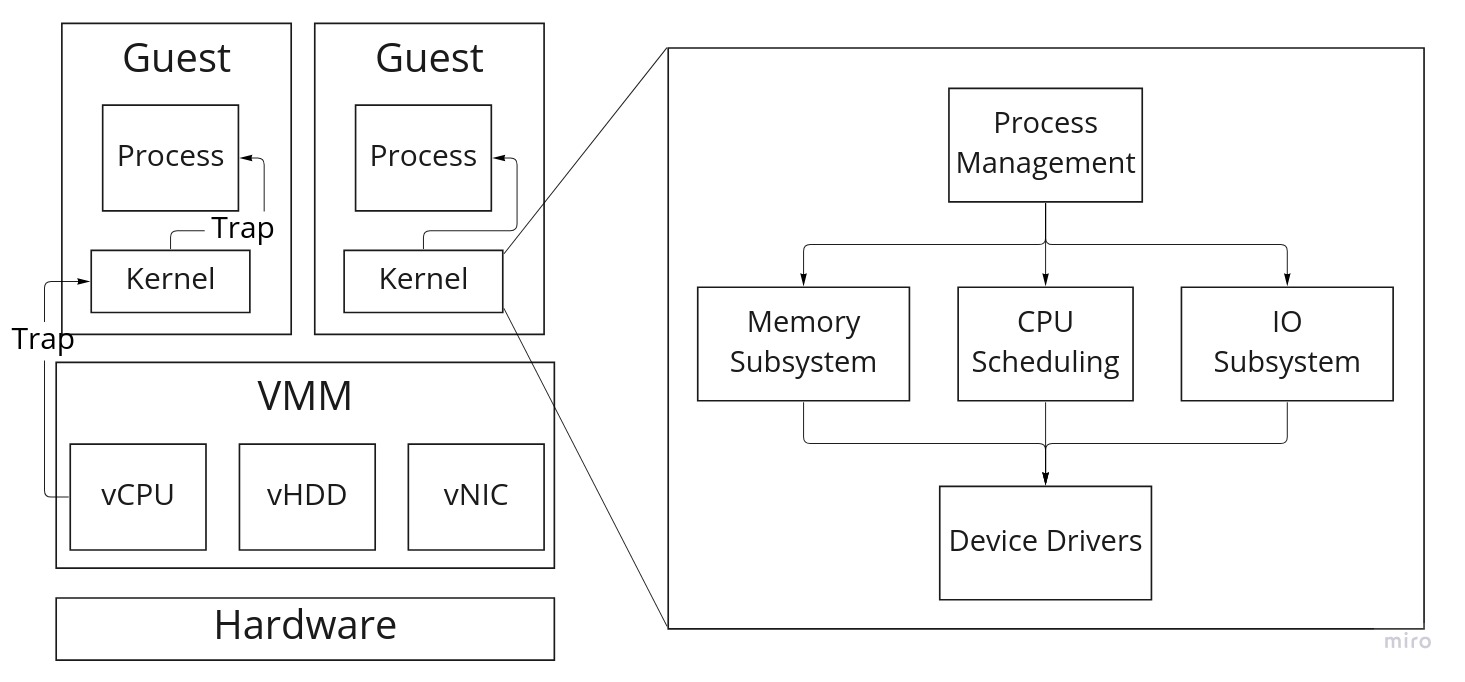
\includegraphics[width=0.70\textwidth]{images/fundamentals/full-virt-archh.jpg}
    \caption{Hardware virtualisation architecture. Each guest runs a complete operating system. 
             Privileged operations are trapped by the virtual machine monitor and emulated to provide hardware services.}
    \label{images:fundamentals/full-virt-archh.jpg}
\end{figure}

\textcite{10.1145/361011.361073} define a requirement that the instruction-set architecture of a computer
has to satisfy for it to be virtualisable. The instruction set must be segregated into three groups of
instructions - privileged, sensitive and innocuous. An instruction is privileged if it requires changing
the mode of execution from user to supervisor mode by means of a trap \cite{10.1145/361011.361073}. 
An instruction $i$ is control-sensitive if, when applied to the current processor state $S_1$, results
in a new state $i(S_{1}) = S_{2}$ such that the execution mode of $S_{2}$ does not equal that of $S_{1}$
or if $S_{2}$ has access to different resources than $S_1$ or both \cite{10.1145/361011.361073}. 
An instruction is behaviour-sensitive if its execution depends on the execution mode or its position
in memory \cite{10.1145/361011.361073}. An instruction is innocuous if it is not sensitive. 
Given these definitions, a computer is virtualisable \enquote{[...] if the set of sensitive instructions
for that computer is a subset of the set of privileged instructions} \cite[6]{10.1145/361011.361073}.
If this criterion is met, the virtual machine monitor can trap all sensitive instructions and emulate 
each via a homomorphism $i: C_{r} \rightarrow C_{v}$ that maps the state space of the processor without
the virtual machine monitor loaded $C_{r}$ to the state space with the virtual machine monitor loaded 
$C_{v}$ \cite{10.1145/361011.361073}. Innocuous instructions do not require protection, i.e a homomorphic
mapping, and are directly executed by the processor \cite{10.1145/361011.361073}.

Given the aforementioned homomorphism, a virtual machine can host a \textit{guest kernel} (Figure \ref{images:fundamentals/full-virt-archh.jpg}) that 
runs completely in user mode. 
Whenever the guest kernel attempts to execute a privileged instruction, 
the virtual machine monitor traps the attempt and emulates the instruction. 
Consequently, the guest kernel does not have to be a part of the trusted computing base. 
Even if it is compromised or encounters an unrecoverable error condition, other virtual machines 
remain unaffected. As a result, the isolation boundary between user programs running in different 
virtual machines is stronger compared to processes running on a shared kernel. 

In order to fully guarantee spatial noninterference between processes, the virtual machine monitor must 
be in full control of the host system's memory. There are two primary methods to do this - 
\textit{shadow paging} and \textit{extended page tables}. The former mechanism is considered first. 
The virtual machine monitor maintains a nested page table 
per guest, also called a \textit{shadow page table} \cite{10.5555/1204009}. 
In turn, the guest kernel maintains a page table per process. 
Whenever the guest kernel schedules a new process for execution, it modifies the \textit{page-table 
base register} to point to the page table for that process \cite{10.5555/1204009}. 
The virtual machine monitor intercepts this attempt and transparently updates the page table pointer to point to 
the guest's shadow page table corresponding to that process \cite{10.5555/1204009}. Note that 
the virtual machine monitor has to traverse the shadow page table for that guest in order to find the nested entry corresponding 
to the process. Afterwards, the memory management unit takes care of translating the virtual memory 
addresses of the guest and updating the \textit{translation lookaside buffer}.
Alternatively, the memory management unit may be \enquote{virtualisation-aware} in the sense that it knows 
there are two page tables it needs to traverse - the page table that maps guest virtual memory to guest 
\enquote{physical memory}, and the page table that maps guest physical memory to actual physical memory. 
The former is maintained by the guest kernel, whilst the latter is maintained by the virtual machine monitor.
The extended page table approach is up to 50\% faster than shadow paging \cite{2006PerformanceEO} because table
walks are done in hardware - by the memory management unit.
Nevertheless, maintaining page table data structures inside the virtual machine 
monitor and the guests leads to memory pressure, which is further amplified by the fact that 
guests, their applications and the virtual machine monitor all share the same physical memory \cite{10.5555/2490781}. 

The spatial noninterference property necessitates that the virtual machine monitor manage 
all input-output devices and their interactions with the guests. This is accomplished by the
already introduced trap-and-emulate pattern. When an application within a virtual machine 
issues a system call requesting some form of input-output, the request is processed by the 
I/O stack inside the guest. At the lowest level of the stack, the device driver issues a 
command to the device, typically by writing to memory specifically assigned to the device, or by
calling specific input-output instructions \cite{10.5555/2490781}. 
Either way, the virtual machine monitor intercepts this and traverses its own I/O stack, which 
remaps guest and real input-output addresses and forwards the request to a physical device \cite{10.1145/2063176.2063194}. 
After processing the request, the physical device triggers an interrupt that is caught by the virtual machine monitor and 
transformed into a virtual equivalent that is sent to the virtual machine that issued the request.
To reduce the overhead associated with interrupt processing, the virtual machine monitor can batch 
multiple events together and use a single interrupt to notify the guest kernel \cite{10.1145/2063176.2063194}.
Still, a request must traverse two input-output stacks. The same holds for the response.
In addition, hardware optimisations such as direct memory access are emulated in software, which 
further degrades performance. This, however, can be mitigated by integrating an input-output memory management 
unit that remaps all direct memory accesses of a device on the host to an address space in the guest.

The cost of hardware virtualisation becomes apparent when measuring same-host density
and boot times. \textcite{10.1145/3132747.3132763} consider memory consumption and on-disk image size
as the primary limiting factors. The authors measure the time it takes to create and boot
virtual machines using the Xen virtual machine monitor and show the negative effects that on-disk image size has 
by starting images with 
varying sizes by manually \enquote{[...] injecting binary objects into the uncompressed image file} \cite[3]{10.1145/3132747.3132763}. 
As the number of consolidated virtual instances increases and the image size grows, 
creation and boot times increase linearly.
Furthermore, the authors show that creating and starting a process directly on the host is, on average, 
two orders of magnitude faster. \textcite{10.1145/2151024.2151030} also evaluate Xen and state
that processing units spend 25\% of their total cycles in hypervisor mode instead of executing guest applications 
when running \enquote{[...] SPEC's first benchmark addressing performance evaluation of datacenter servers used in 
virtualised server consolidation} \cite[2]{10.1145/2151024.2151030}, which includes components 
such as a web, database and application server.

\subsection{Operating System Virtualisation}
\label{ch:fundamentals/virtualisation/os-virtualisation}
\textit{Operating system virtualisation} refers to all mechanisms that enable the creation of secure
and isolated application environments that run on top of a shared kernel. 
Conventionally, these mechanisms are baked into the kernel and are therefore part of the trusted computing base.
The kernel may expose these through its system-call interface, thereby allowing a user-space daemon 
program to provide an automated facility for creating and orchestrating sandboxed environments. 
This is the only feasible architecture on a general-purpose kernel such as Linux. 
Alternatively, the kernel may treat every software component, including its own subsystems, as an entity
to be wrapped in a sandbox. In that case, the concept of a process itself would have to 
satisfy all three virtualisation axioms. Examples of such operating systems include the seL4 \textit{microkernel}
- the first operating system to be formally verified as free of programming errors \cite{10.1145/1629575.1629596}, 
and Google's Fuchsia - described by \textcite{10.22667/JOWUA.2021.09.30.047}.

We only consider operating system virtualisation using a user-space daemon program.
In this architecture, an application, referred to as a \textit{container},
is defined as an encapsulation of \enquote{[...] a software component and all its dependencies 
in a format that is self-describing and portable, so that any compliant container runtime can run it without extra 
dependencies, regardless of the underlying machine and the contents of the container} \cite[1]{oci-runtime-principles}.
A \textit{container runtime} is the user-space daemon program responsible for bringing this portable but 
static representation of an application into execution. In runtime, a container consists of a collection of processes 
that share a restricted view of the system's resources. For example, every container \enquote{believes}
it has a dedicated network stack with its own network interfaces, routing tables and packet-forwarding rules.
All processes in the container can access and manipulate that network stack, but no other process 
outside the container has that capability.
The container runtime configures this invariant and the operating system enforces it by 
namespacing system resources. The Open Containers Initiative (OCI) \cite{oci-website} has 
developed a runtime specification that standardises the operations a container runtime
needs to support. Most importantly, it must allow an external process called a \textit{container engine}
to hook into the lifecycle of a container. The container engine can use these hooks to manage 
all the containers on a single host system. In addition, the engine can attach network and storage 
to containers, thereby allowing processes in different sandboxes to share state and communicate 
with each other, if required. At the highest level of abstraction sits an orchestration platform that 
manages containers on multiple hosts by interacting with the container engine on each system.
This platform constantly monitors node and container health and dynamically multiplexes workloads 
based on various system properties of the cluster as to ensure maximum application availability.

It is important to note that, by definition, the kernel is assumed to be trustworthy. 
It has full control of all hardware resources and can access and modify the execution environment of every process on the system. 
In other words, noninterference between the kernel and user processes is not guaranteed.
Therefore, if the kernel is compromised, all processes on the system become untrustworthy.
It follows that if a process compromises the kernel, it transitively interferes with all other 
processes on the system. Hardening the operating system by implementing various security features such as
mandatory access control has been the primary approach for protection against such scenarios. 
However, the size of a monolithic general-purpose kernel is too large to adequately 
create a threat model that captures all possible vectors of attack. This problem is of particular concern 
to infrastructure providers whose entire business model revolves around consolidating hundreds of potentially 
malicious client applications on the same server, all of which share the same kernel and are allowed to directly interact with 
it via its system call interface. 

Unlike hardware virtualisation, this architecture does not use hardware emulation as an 
isolation primitive.
This means that shadow pages need not be maintained per virtual environment. Input-output operations need only 
traverse the kernel's stack without any address translations and with the additional 
performance benefit of direct memory access. As a result, the isolation overhead is lower 
compared to a virtual machine, which allows more applications to be consolidated onto a single server.
Furthermore, guests do not boot up complete operating system images, which reduces 
start times and memory consumption.
\textcite{10.1145/3126908.3126925} use containers in high-performance 
computing clusters to run user-defined compute jobs and show that the imposed performance penalties 
are, at most, negligible compared to vanilla processes that have no additional isolation.
\textcite{7095802} show the exact same thing and further conclude that the Docker container engine 
is resource-friendlier and faster than the Kernel Virtual Machine (KVM) when stressing the
\enquote{memory, IPC, network and filesystem subsystems} \textcite[1]{7095802} of the Linux kernel 
by running a database inside a virtual environment and evaulating its performance via the SysBench OLTP benchmark \cite{sysbench-oltp}.

Google's gVisor \cite{google-gvisor} attempts to sustain the performance advantages of 
containers whilst introducing an additional isolation boundary between the kernel and each container. The authors implement 
a substantial portion of the system call interface in a user-space process called Sentry.
Their dedicated container runtime calls out to Sentry instead of the kernel when issuing system calls.
\begin{figure}[H]
    \centering
    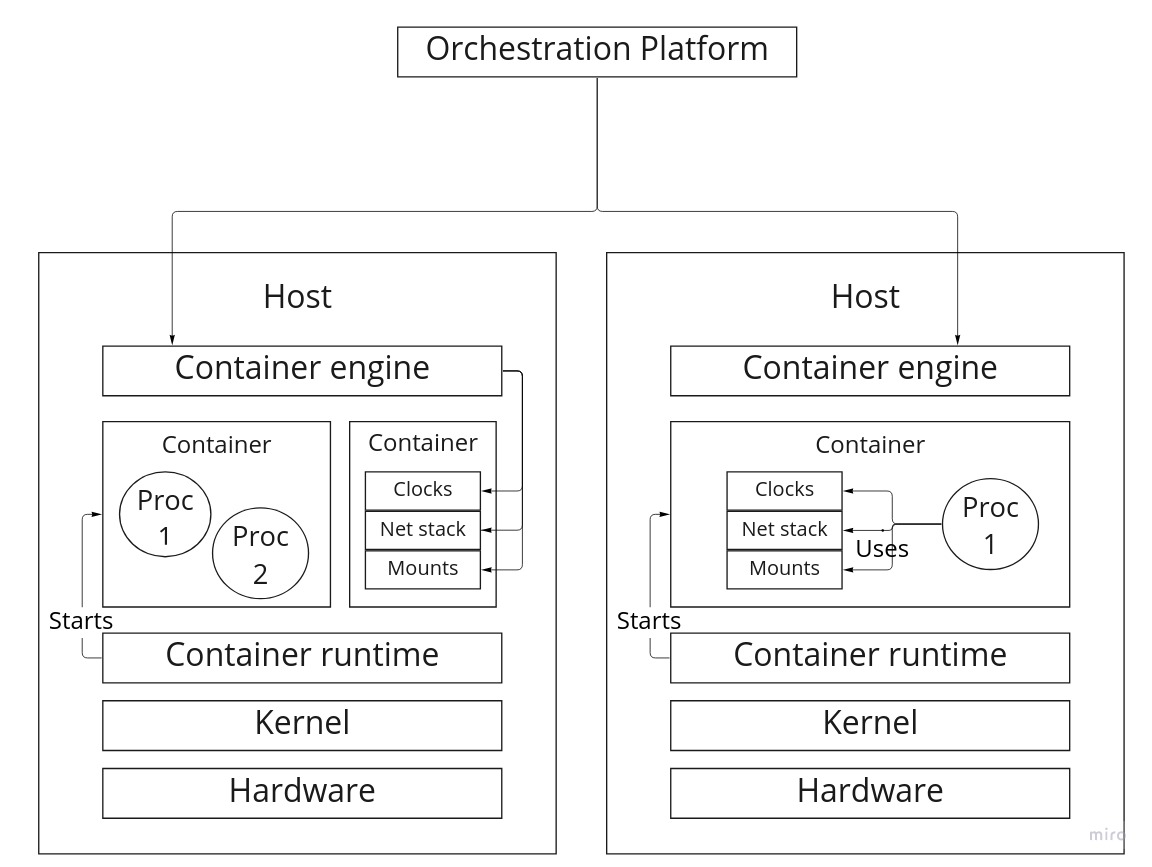
\includegraphics[width=0.55\textwidth]{images/fundamentals/cont-arch.jpg}
    \caption{Operating system virtualisation architecture using containers. The container runtime starts containers on a single host.
    A user process can see a bundle of resources allocated to it by the kernel. The kernel guarantees that a process 
    cannot see any other resources.
    The container engine manages all containers on a single system and allocates storage and networking to create explicit paths between containers.
    The orchestration platform talks to all engines inside a cluster to provide automatic workload management.}
    \label{images:fundamentals/cont-arch.jpg}
\end{figure}
However, \textcite{234857} show that network and memory allocation performance greatly suffer. 
This can be partially attributed to the fact that the Sentry process is implemented in a garbage-collected language 
and lacks the fine-grained optimisations contained in the Linux kernel.
\textcite{246288} take a different approach and try to fuse the security of virtual machines 
with the performance of containers by programming a custom virtual machine monitor 
called Firecracker that runs on top of KVM. Firecracker completely relies on the
Linux kernel for memory management, CPU scheduling and block I/O. To reduce its attack surface,
the virtual machine monitor sacrifices portability by supporting a limited set of emulated 
network and block devices. To further strengthen the noninterference boundary, the devices 
have configurable built-in rate limiters that can control the number of operations per second, e.g
disk/packets per second. Unlike a traditional container runtime, Firecracker's rate-limiting implementation
does not rely on the kernel, which makes its isolation boundary to the kernel stronger. 
\textcite{10.1145/3381052.3381315} evaluate both gVisor and Firecracker and show that 
the latter \enquote{[...] is effective at reducing the frequency of kernel code invocations, but had 
a much smaller impact on reducing the footprint of kernel code} \cite[12]{10.1145/3381052.3381315}. 
\clearpage

\section{Processes}
\begin{figure}[H]
    \centering
    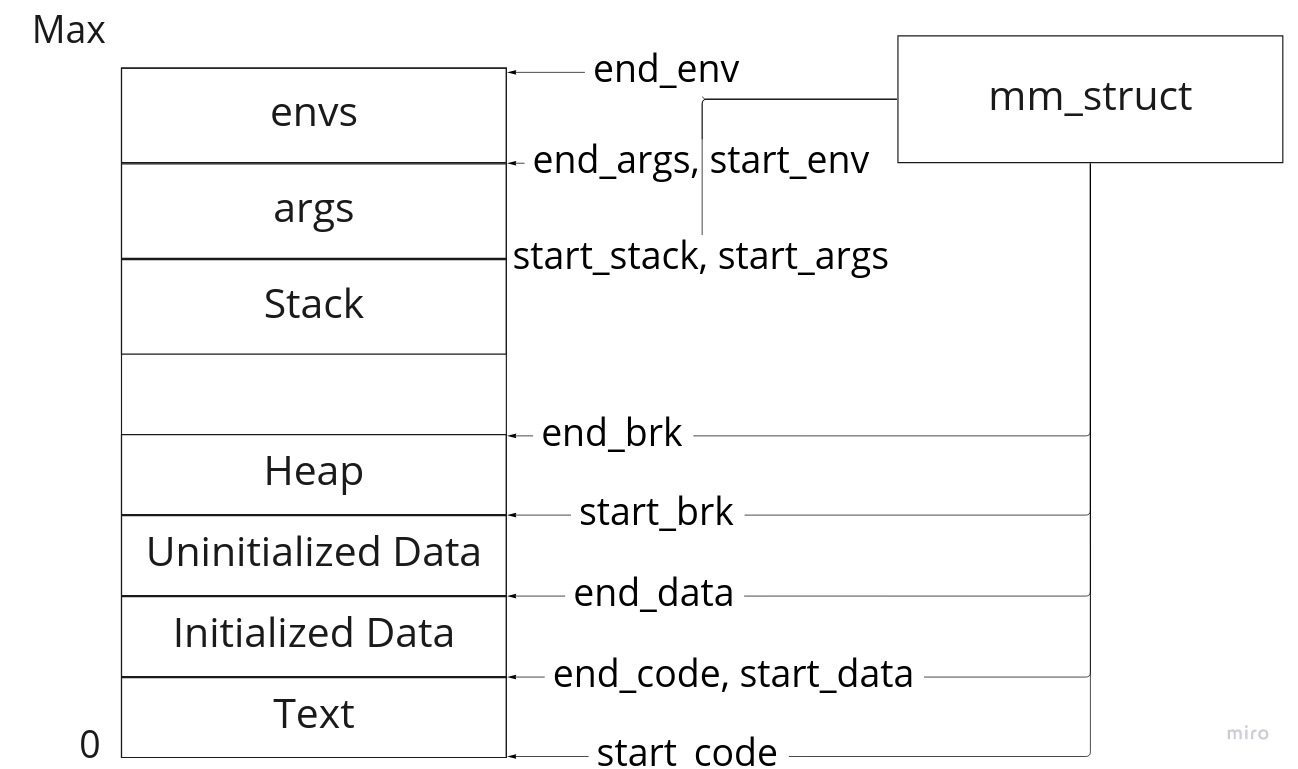
\includegraphics[width=0.6\textwidth]{images/fundamentals/proc-mem-layout.jpg}
    \caption{Memory layout of a process \cite{10.5555/2490781}}
    \label{images:fundamentals/proc-mem-layout}
\end{figure}

A process is the fundamental abstraction of operating-system virtualisation.  
It is the primary unit of work in a computer system and represents a program in execution.
This chapter introduces various aspects of a process - how it is laid out in memory 
(Chapter \ref{ch:fundamentals/processes/memory-layout}), how it is scheduled for execution 
(Chapter \ref{ch:fundamentals/processes/execution-scheduling}), and the system call interface for 
creating, terminating, monitoring and protecting processes from each other 
(Chapters \ref{ch:fundamentals/processes/creation}, \ref{ch:fundamentals/processes/termination},
\ref{ch:fundamentals/processes/monitoring}, \ref{ch:fundamentals/processes/resource-management}, 
\ref{ch:fundamentals/processes/security}).

Every process on Linux is represented as a \verb|task_struct| \cite{include/linux/sched.h} 
which contains various bits of information such as the process's memory descriptor, the table of 
open file descriptors, the running state of the process (see Table \ref{table:proc-states}), 
its pending signals and so on.
Processes are organised in a hierarchy, where each process can have an arbitrary number of children
and a single parent. The kernel expresses this relationship by having each task store a pointer 
to its parent and a circular doubly linked list to all of its children. 

\subsection{Memory Layout}
\label{ch:fundamentals/processes/memory-layout}
The kernel partitions the virtual address space of a process into multipe regions shown in Figure 
\ref{images:fundamentals/proc-mem-layout}. The address space itself is encapsulated in a 
memory descriptor type called \verb|mm_struct| \cite{include/linux/mm_types.h} and 
every process is associated with one or more instances of that type. The text 
segment of the address space is a read-only memory section that contains the set of executable 
instructions that the program compiles down to \cite{10.5555/2490781}. When the program is 
first scheduled for execution, the central processing unit jumps to the text section's 
initial memory address, which is stored in the \verb|start_code| field of the process's memory descriptor
and starts executing from there until it reaches the final linear address \verb|end_code|.
The data section contains globally defined variables that can be referenced throughout the 
entire lifecycle of the process \cite{10.5555/2490781}. The data section is further deconstructed 
into uninitialised and initialised subsections. Similarly to the text section, it
does not grow or shrink because its size is known at program startup and does not change. 
The \verb|start_data| and \verb|end_data| fields in the memory descriptor refer to the 
contiguous memory region that represents the initialised data. 
The heap segment contains memory that is allocated during runtime as per demand. The process 
itself is responsible for releasing any memory acquired from the heap. The latter is important for two 
reasons. First, the heap grows upwards towards the stack and may overlap with it. Second, 
memory allocation interfaces such as \verb|malloc| acquire memory from a system-wide pool. If a 
long-running process acquires dynamic memory but fails to release it, the whole system will 
eventually run out of memory - an example of spatial interference. The kernel tracks the heap areas 
allocated to a particular process via the \verb|start_brk| and \verb|brk| fields of the memory 
descriptor which denote its initial and final linear addresses, respectively. 
The stack is a data structure that acts as temporary storage for a process. Whenever 
a process calls a function, that function's parameters, local variables and return address are pushed 
onto the stack. When the function returns control to the caller, these values are popped of \cite{10.5555/2490781}.
The stack grows downwards towards lower addresses and its starting address \verb|start_stack|
sits right above the \verb|main()| function's return address. 

Note that the virtual address space of the process is sparse because it contains a hole between the 
stack and the heap that will require physical pages only if those two segments grow. This hole may be
utilised to bring in page frames that can be shared between processes in order to reduce memory 
consumption and to allow two processes to communicate with each other. For example, the \verb|libc|
library is reentrant and can be brought into physical memory only once. The memory descriptor of a 
process that depends on \verb|libc| does not have to load its own copy of the library into memory. 
Instead, its page table entries can map to the same physical frames that all other processes refer to 
when using the library. This reduces memory consumption and therefore has positive implications 
on same-host density.

\subsection{Scheduling}
\label{ch:fundamentals/processes/execution-scheduling}
Systems running more than one process rely on a process scheduler to determine, in real-time, 
which process should use the processing unit such that all processes do meaningful work 
and the core does not idle. 
The process scheduler maintains a  queue of all processes that are currently 
being executed by a processing unit or are waiting to be assigned to one. 
This queue is represented in memory as a circular doubly linked-list of \verb|task_struct| 
objects and is called the run queue because all of its tasks are in the \verb|TASK_RUNNING| state.
The kernel keeps a run queue local pointer \verb|current| to the current task being executed by a processing unit. 
It is the scheduler's job to determine the most optimal sequence of processes to schedule from the run queue 
onto the processing unit in order to satisfy two conflicting requirements - low latency and high throughput. 
Low latency is crutial for processes that mostly perform input-output operations. 
Fetching data from a device, such as a network card, typically takes multiple CPU cycles. 
For this reason, the scheduler moves a task currently waiting for an external event from the running queue 
into the wait queue and updates the \verb|current| pointer to point to a different process. 
This operation is known as preemption. 
\begin{table}[h!]
    \centering
    \begin{tabular}{ |m{4cm}|m{20em}| }
        \hline
        State identifier & Description \\
        \hline
        \verb|TASK_RUNNING| & The process is being executed by a CPU or is waiting to be assigned to one \\
        \hline 
        \verb|TASK_UNINTERRUPTIBLE| & The process is waiting for an event or a resource and cannot be interrupted by a signal while doing so \\
        \hline
        \verb|TASK_INTERRUPTIBLE| & The process is waiting for an event or a resource and can be interrupted by a signal while doing so \\
        \hline
        \verb|TASK_NEW| & The process has been created but it cannot be scheduled for execution and it cannot react to events \\
        \hline
        \verb|EXIT_DEAD| & The process is being cleaned up and deleted \\
        \hline
        \verb|EXIT_ZOMBIE| & The process has exited, the parent has been notified via a \verb|SIGCHLD| signal but the parent has not reaped it yet \\
        \hline
    \end{tabular}
    \caption{Table of most important process states in Linux derived from \cite{include/linux/sched.h} and \cite{kernel/sched/core.c}}
    \label{table:proc-states}
\end{table}
The wait queue consists of all processes currently waiting for data or a signal.
Their state is always either \verb|TASK_INTERRUPTIBLE| or \verb|TASK_UNINTERRUPTIBLE|.
In order for an input-output bound process to make meaningful progress, it needs to be frequently 
rescheduled back onto the processing unit. 
Conversely, high throughput is important for processes that are primarily executing computations.
These processes make the most progress by monopolising the processing unit. Hence, 
low-latency and high throughput are incongruous. Operating systems manage 
this incongruity by ranking processes based on their priority and allocating timeslices that 
determine how long a task can run until it is preempted.

On Linux, every \verb|task_struct| is associated with a \verb|sched_entity| object that holds task-related 
statistics used by the scheduler to do its job. The most important properties of this object 
are the \verb|weight| and \verb|vruntime| fields. The former represents 
a priority value that measures the task's willingness to be preempted. In other words, it represents 
how \enquote{nice} a process is to all other processes on the system. The value ranges from $-20$
to $19$ with a default of $0$. Larger values correspond to lower priorities and smaller values correspond 
to higher priorities. The \verb|vruntime| (virtual runtime) field denotes the amount of time already 
allocated to the task. The invariant that the scheduler tries to enforce is that the process with the 
smallest virtual runtime should be the one that is currently using the processing unit. By definition,
the process with the smallest virtual runtime is also the process that has used the processing unit
the least. For this reason, the scheduler is said to be completely fair. 
Whenever the run queue is updated, either by an interrupt triggered by the system timer or a 
change in a task's state, the virtual runtime of the task is incremented by a weighted delta
\begin{equation}
    d = e \times w / \sum_{i = 0}^{n} w_{i}
    \label{equation:fundamentals/cfs-scheduler-delta}
\end{equation}
where $e$ refers to the amount of time the task used the central processing unit 
since the last time the run queue was updated. 
$w$ corresponds to the priority value of the task. $n$ denotes the length of the run queue. 
The sum in the expression aggregates the priority values of all tasks in the queue. 
Hence, dividing $w$ by the sum gives us a proxy of the task's priority relative to all 
other tasks in the queue. Recall that the scheduler monotonically increases the virtual runtime 
of the process by $d$. A process that performs a lot of input-output operations exhibits small 
processing unit bursts, hence $e$ is smaller. Therefore, the virtual runtime for that process 
will increase more slowly and the process will be scheduled more frequently for execution. 
Similarly, if the process has a high priority, i.e $w$ is small, 
the division in Equation \ref{equation:fundamentals/cfs-scheduler-delta} will result in a small fraction 
that will cancel out a big portion of $e$ when multiplied. 

The \verb|sched_entity| object of every process is a part of a 
a red-black tree whose search key is set to the virtual runtime property. The scheduler picks a new process 
for execution by traversing the tree and finding the task with the lowest virtual runtime, which is always 
stored at the leftmost leaf node. The cost of traversal equals the depth of the tree, i.e it takes $\Theta{(\log{n})}$.
However, the scheduler caches the leftmost node, thereby reducing the cost of traversal down to $\Theta{(1)}$.
Whenever a process transitions from the \verb|TASK_NEW| state into the \verb|TASK_RUNNING| state, 
it is assigned the minimal allowed virtual runtime. Therefore, it is automatically 
placed at the leftmost node and gets to execute immediately. As the system progresses, the process will
shift more and more to the right branches of the tree and the rest of the tasks will get to execute.

\subsection{Creation}
\label{ch:fundamentals/processes/creation}
The \verb|libc| wrapper functions \verb|clone()| and \verb|fork()| are the only mechanisms for 
creating a new process from user space. The former is a non-portable but very flexible method for creating a
duplicate of the calling process. It gives the caller fine-grained control over the resources that 
the parent and the child get to share. Both functions internally use the \verb|SYS_clone| system call 
to create the child. However, \verb|clone()| gives the caller the ability to configure the child's execution 
context, whereas \verb|fork()| does not. Instead, \verb|fork()| transparently preconfigures the child.
It is important to note that the the configuration options passed into \verb|SYS_clone| define 
the noninterference boundary between a child and its parent. As a matter of fact, the 
noninterference boundary is what allows us to differentiate between a process and a thread. 
A child whose memory descriptor refers to the same virtual memory pages as its parent is a thread. 
A child with separate virtual memory pages is a process. 
\clearpage

\begin{lstlisting}[style=syscalls, caption={Clone and Fork System Call Wrappers}]
#define _GNU_SOURCE
#include <sched.h>

int clone(int (*fn)(void *), void *stack, int flags, void *arg, ...
          /* pid_t *parent_tid, void *tls, pid_t *child_tid */ );

/* Returns thread id of child on success, -1 on error with errno set */

#include <unistd.h>

pid_t fork(void);

/* Returns process identifier of child in parent, or -1 on error; Returns 0 in child */

\end{lstlisting}
Whenever a new child process is created, both the parent and the child share the same text segment.
The child obtains a dedicated copy of the parent's stack, heap and data segments if and onl if 
it attempts to write to one of those segments. Otherwise, the kernel will not explicitly copy 
anything, due to the expensivness of the operation. This technique is known as copy on write.

\verb|clone()| creates a child process that begins its lifecycle by executing 
the function pointer \verb|fn|. The return value of \verb|fn| represents the exit code with which 
the child process will terminate. The function pointer expects a generic argument 
as input that can be concretised by the caller via the \verb|arg| parameter.
The \verb|flags| argument represents a bit mask used by the caller to configure 
the child's execution context. For example, setting the \verb|CLONE_VM| flag will result in 
both processes sharing the same virtual address space. Memory writes performed by one process will 
be visible to the other process. Similarly, the \verb|CLONE_FILES| flag can be set so that 
the child and parent processes share the same file descriptor table. If one of the processes 
closes a file descriptor, the other process is also affected. The bit mask can also be used 
to put the child process in freshly-allocated resource namespaces - an important noninterference construct 
discussed in Chapter \ref{ch:fundamentals/processes/security}. The lower byte of the bit mask 
is used to specify the child's termination signal. If left unset, the parent has no way 
of reaping the child.

The caller is expected to provide a memory region to be used as the new process's stack. 
The system call wrapper pushes the function pointer onto the stack and transfers execution 
to the kernel. The kernel creates the new process by copying the old process - taking into consideration 
which parts should be copied based on the \verb|flags| bit mask. Importantly, the kernel places 
the start address of the user-defined stack into the stack register of the processing unit.
Afterwards, the process is placed in the run queue and control is returned to the system call wrapper.
The system call itself returns two times - once in the parent process where the return value corresponds 
to the process identifier in the child, and once in the child process where the return value is zero. 
The system call wrapper handles the latter case by popping the function pointer of the stack 
and calling it \cite{aarch64/clone.S}, thereby using the function pointer as the main entry point 
into the child process.

There are multiple caveats that need to be considered when calling \verb|clone()|. 
First, the \verb|stack| parameter must point to the top address of the stack. Because the stack 
grows downwards, the address to be passed to \verb|clone()| is not the start address of the memory region but the 
end address, which needs to be aligned according to the application binary interface. Second, 
careful attention must be paid when creating a child with the \verb|CLONE_VM| flag set. 
The child process cannot depend on anything defined in \verb|libc| because it risks polluting 
the parent's runtime environment. In particular, important variables allocated in thread-local storage 
by the linker are not set up for the child, e.g the \verb|errno| variable, the standard input-output streams
and more. Instead, they are shared between parent and child. 

\subsubsection{Example 1}

Code snippet \ref{code:os-concepts/src/clone.c} shows how to create a child process via 
the \verb|clone()| wrapper. First, the parent prints its process identifier to standard output. 
Afterwards, it sets up a memory region to be used as the child's stack by allocating 
two pages of memory that can be read from and written to by both processes.
The memory region is not backed by external storage and changes made by one process are not visible to the other.
Furthermore, the starting memory address is page-aligned and chosen by the kernel.
On line 22, the system call wrapper is executed with the \verb|child_process| function set as the entry point into the child. 
The \verb|shared_resources| variable refers to the 
bit mask that controls what the parent and child get to share. It is set to zero, indicating that 
they will not share any resources. The bit mask is ORed with \verb|SIGCHLD| - the signal 
that will be sent to the parent when the child finishes execution. On lines 27-31, the 
parent blocks until it receives the \verb|SIGCHLD| signal  from the child and exits.
In (\ref{code:os-concepts/src/clone.c-exec}) the output of the program shows the 
relationship between the child and the parent obtained by calls to \verb|getpid()| and \verb|getppid()|. 

If we were to modify the example in (\ref{code:os-concepts/src/clone.c}) so that the parent and child share the same virtual memory pages,
then thread-local variables would not be properly 
placed in thread-local storage, potentially 
resulting in undefined behavior when interacting with \verb|libc|.

The \verb|fork()| system call creates a child process transparently preconfigured to share 
no resources with the parent and to respond to the \verb|SIGCHLD| signal upon termination.
In other words, it is equivalent to calling \verb|clone()| with the \verb|flags| bit mask set to 
zero and ORing it with \verb|SIGCHLD|. \verb|fork()| returns two times - once in the parent and once in the child. In the latter 
case, the returned value is zero. Hence, the caller can define the child's logic via a conditional 
statement.

\lstinputlisting[label={code:os-concepts/src/clone.c}, style=c-code-snippets, caption={os-concepts/src/clone.c}, firstline=13, lastline=47]
{/home/nas/lxc-research/src/os-concepts/src/clone.c}
\begin{lstlisting}[label={code:os-concepts/src/clone.c-exec}, style=bash, caption={os-concepts/src/clone.c output}]
    $ ./clone 
    Parent: 329638
    Child: 329657
    Child parent: 329638
\end{lstlisting}

\subsection{Termination}
\label{ch:fundamentals/processes/termination}
\begin{lstlisting}[style=syscalls, caption={Exit System Call and Wrappers}]
#include <stdlib.h>

noreturn void exit(int status);

int atexit(void (*function)(void));

/* Returns 0 if successful; otherwise a nonzero value */

#include <unistd.h>

noreturn void _exit(int status);
\end{lstlisting}

Processes can terminate abnormally or normally. Abnormal termination happens when a process 
receives a signal from the kernel or another process. For example, division by zero causes 
the hardware to detect a fault condition and notify the kernel. The kernel can then send a termination 
signal to the process that made the arithmetic error. Sending a signal to a process directly 
interrupts its execution flow by saving the current state of the registers and causing the processing 
unit to jump to a signal handler - a function dedicated to processing a particular signal. 
After the signal handler is executed, the process either terminates or continues its execution from 
the point of interruption. 

A process terminates normally when it invokes the \verb|_exit()| system call. In doing so, it notifies the 
kernel that it can reclaim all of the process's resources, including its memory descriptor, 
file table, scheduling information and more. Additionally, the kernel notifies the parent 
about the child's termination by sending it the termination signal defined when the child was created - 
typically the \verb|SIGCHLD| signal. The child can send its termination status to the parent
by passing a signed integer to the \verb|_exit()| functon. Conventionally, an exit status of 0 
means that the child has successfully executed its operations.

Alternatively, a process can call the \verb|exit()| wrapper defined in \verb|libc|, which internally 
uses \verb|_exit()|.
In addition to releasing operating-system resources, the \verb|exit()| function also invokes 
a set of exit handlers defined by the application programmer and \verb|libc| to cleanup auxillary
resources. For example, \verb|libc| defines an exit handler that flushes the standard input-output 
buffers of the process. Users can register exit handlers via the \verb|atexit| function. 
Exit handlers are called in reverse order of registration. If an exit handler fails to return, then 
the remaining set is not called. 

\subsubsection{Example 2}
\begin{lstlisting}[label={code:os-concepts/src/exit-normal.c}, style=c-code-snippets, caption={os-concepts/src/exit-normal.c}]
void exit_handler_1(void)
{
    printf("Process %d invoked exit handler 1\n", getpid());
}
void exit_handler_2(void)
{
    printf("Process %d invoked exit handler 2\n", getpid());
}
int main(int argc, char *argv[])
{
    printf("Parent process: %d\n", getpid());
    /* Register exit handlers in parent */
    atexit(exit_handler_1);
    atexit(exit_handler_2);
    pid_t child = fork();
    if (child < 0)
        goto err;
    if (child == 0) {
        /* Child process begins execution here */
        printf("Child process: %d\n", getpid());
        exit(0);
    }
    int status;
    if (waitpid(child, &status, 0) != child)
        goto err;
    printf("Child exited with status %d\n", status);
    return 0;
err:
    printf("%s", strerror(errno));
    return 1;
}
\end{lstlisting}
\begin{lstlisting}[label={code:os-concepts/src/exit-normal.c-exec}, style=bash, caption={os-concepts/src/exit-normal.c output}]
    $ ./exit 
    Parent process: 14862
    Child process: 14863
    Process 14863 invoked exit handler 2
    Process 14863 invoked exit handler 1
    Child exited with status 0
    Process 14862 invoked exit handler 2
    Process 14862 invoked exit handler 1
\end{lstlisting}
Code snippet \ref{code:os-concepts/src/exit-normal.c} shows an example of normal process termination. 
The parent registers two exit handlers that print the identifier of 
the process that invoked them. On line 19, the parent creates a child via the \verb|fork()| system call.
The child prints its process identifier and invokes \verb|exit()| with a status of zero. This causes 
the kernel to send a notification signal to the parent who is waiting at line 30 until it receives 
the signal. The parent prints the status of the child and exits. In (\ref{code:os-concepts/src/exit-normal.c-exec}) the program 
is executed. Notice that the exit handlers are invoked four times - two times in the parent and two times 
in the child. That is because a child inherits a copy of its parent's exit registrations. 
Since the child exits first, it always invokes the exit handlers before the parent.
If the child had terminated via \verb|_exit()|, then the exit handlers would have been executed 
solely by the parent.

\subsubsection{Example 3}
Code snippet \ref{code:os-concepts/src/exit-abnormal.c} shows an example of abnormal process termination 
caused by an interactive interrupt signal. The parent creates a child that registers a signal handler 
to be executed whenever it receives a \verb|SIGINT| signal. The signal handler is registered via the 
\verb|sigaction| system call, which overrides the default handler for \verb|SIGINT| with the one 
specified in the \verb|.sa_handler| field. 
The signal handler prints a message to
standard output and terminates the process.
After registering the handler, the child suspends itself, i.e it manually enters the \verb|TASK_INTERRUPTIBLE| state by 
calling \verb|pause()|. 
On line 27, the parent waits for the child to exit. 
If the child does not receive a \verb|SIGINT| signal, the parent will wait indefinitely.
The program is executed in (\ref{code:os-concepts/src/exit-abnormal.c-exec}) by starting the parent as a background task and 
manually sending the \verb|SIGINT| to the child process through the \verb|kill| command.  
The signal handler that terminates the child is triggered and the kernel notifies the parent of the event.
The parent reports the child's termination status and exits. 

It is important to note that calling \verb|printf| from a signal handler may be unsafe in certain circumstances.
Consider a thread of execution being interrupted by a signal handler while it is executing \verb|printf|.
If the signal handler also calls \verb|printf|, it will corrupt the internal data structures used to 
keep track of the amount of data and the current position in the buffer. This will lead to 
unexpected results when control is returned back from the signal handler to the thread.
For this reason, the \verb|printf| function is said to be async-signal unsafe, i.e it is not atomic 
with respect to signal interrupts.  In the current example, the child does not call \verb|printf|
after the new signal handler is registered, so its usage is safe. 
In practice, however, processes 
are large and complex enough for this to become a problem. 

Also, signal handlers cannot be used to reliably track the number of signals generated, because 
signals are not queued. While a signal handler is executing and the same signal is sent 
multiple times to the process, that signal is marked as pending and is later redelivered only once.

\begin{lstlisting}[label={code:os-concepts/src/exit-abnormal.c}, style=c-code-snippets, caption={os-concepts/src/exit-abnormal.c}]
/* Will get triggered when the caller pushes Ctrl+C */
void default_interaction_handler(int signal)
{
    printf("Terminating process\n");
    _exit(0);
}
int main(int argc, char *argv[])
{
    pid_t child = fork();
    if (child < 0)
        goto err;
    if (child == 0) {
        printf("Child identifier: %d\n", getpid());
        /* Child registers sigint handler */
        struct sigaction action = {.sa_handler = default_interaction_handler };
        if (sigaction(SIGINT, &action, NULL) != 0)
            goto err;

        /* Child is suspended until it receives a signal */
        pause();
    }
    /* Caller will block indefinitely until child exits */
    int status;
    if (waitpid(child, &status, 0) != child)
        goto err;
    printf("Child exited with status %d\n", status);
    return 0;
err:
    printf("%s", strerror(errno));
    return 1;
}
\end{lstlisting}
\begin{lstlisting}[label={code:os-concepts/src/exit-abnormal.c-exec}, style=bash, caption={os-concepts/src/exit-abnormal.c output}]
$ ./exit-abnormal &
[1] 162043
Child identifier: 162044
$ kill -s SIGINT 162044
Terminating process
Child exited with status 0
[1]+  Done                    ./exit-abnormal
\end{lstlisting}
\subsection{Monitoring}
\label{ch:fundamentals/processes/monitoring}
\begin{lstlisting}[style=syscalls, caption={Wait System Call and Wrappers}]
#include <sys/wait.h>

pid_t wait(int *status);

/* Returns process identifier of terminated child; -1 on error */

pid_t waitpid(pid_t pid, int *status, int options);

/* Returns process identifier of child; 0; -1 on error */
\end{lstlisting}
The parent process often wants to gather information about when and how a child has terminated. 
This functionality is provided by \verb|wait()| and \verb|waitpid()|, as already shown in 
(\ref{code:os-concepts/src/clone.c}), (\ref{code:os-concepts/src/exit-normal.c-exec}) and (\ref{code:os-concepts/src/exit-abnormal.c-exec}).

%The parent is required to reap 
%the child. Otherwise, the identifier of the child will not be removed from the system-wide 
%table of process identifiers.

\subsection{Communication}
\label{ch:fundamentals/processes/communication}
TODO
\subsection{Resource Management}
\label{ch:fundamentals/processes/resource-management}
TODO 
\subsection{Security}
\label{ch:fundamentals/processes/security}
Every process is associated with a set of credentials. 
The traditional UNIX security model defines these credentials 
as a set of unique numerical user and group identifiers. The \textit{real} user and group identifiers 
represent the user to which the process belongs. They are read from the 
password database as part of the login procedure \cite{10.5555/1869911}. 
Every process spawned by the user inherits the real user and group identifiers as part of 
its credentials. 
The credentials themselves further consist of an \textit{effective} user and an effective group identifier,
which are used by the kernel to authorise and execute operations on behalf of the process \cite{10.5555/1869911}.
For example, when a process attempts to read a file, the kernel checks if the effective user ID
of the process matches the user ID of the owner of the file, or if the effective group ID matches the 
owner's group ID. If any of these predicates holds, then the effective user - and therefore the process - 
is deemed trustworthy to call the \verb|read| system call on a file descriptor referencing the file.
Typically, the effective user and group identifiers match their real counterparts. However, there 
are programs that can ambiently change the effective identifiers of a process to match 
those of the user that created them \cite{10.5555/1869911}. These programs are known as 
\textit{set-user-id} and \textit{set-group-id} programs. Every executable file is associated with 
a set-user-id and a set-group-id permission bit that can be set by that file's owner. 
If the set-user-id permission bit is set and another user executes the program, the process
obtains the effective user identifier of the file's owner, not the user that started the process \cite{10.5555/1869911}.
A classic example of a set-user-id program is \verb|sudo|, which executes arbitrary commands as the 
root user. Since the \verb|sudo| executable file is
owned by the root user and has the set-user-id bit toggled, any user cam execute any command 
in a process with full privileges. Another example is the \verb|passwd| utility which allows a user 
to change her password and therefore requires write access to the password database.  

Notice that the UNIX security model differentiates only between privileged and unprivileged processes.
The former are not subjected to permission checking and have full control of the system - they can 
reboot the system, set the system time, kill other processes and so on. 
If a set-user-id or a set-group-id program exhibits unexpected behaviour, either due to malicious manipulation or 
programming errors, this coarse-grained security model is unable to prevent a full system exploitation.
The Linux capability scheme tries to solve this problem by unbinding privileges from the root 
user and dividing them into components called \textit{capabilities}. A capability is represented as 
a single bit that is a part of a 64-bit wide bit mask, called a \textit{capability set}.
Every process is associated with a \textit{permitted}, \textit{inheritable}, \textit{effective}, 
\textit{bounding} and \textit{ambient} capability set. 
%In addition, every executable file may optionally 
%be associated with its own permitted and inheritable sets.
Whenever a process starts a child, that child inherits the capability sets of its parent.
The effective capability set of a process
is used by the kernel to perform permission checks. The permitted capability set acts as a 
superset that restricts the effective capabilities that a process can assume. 
If a process drops a capability from its permitted set, it cannot acquire that capability any more.

Executable files may also be associated with permitted and inheritable capability sets. 
Such files are said to be privileged. 
Whenever a process loads an executable into memory, the permitted and inheritable capability 
sets of the file interact with those of the process to determine the process's new set 
of capabilities. We denote a process that has not loaded an executable file as $P$, the executable 
file as $F$ and the process with the executable file loaded as $P^{\prime}$. 
\begin{align}
    P^{\prime}(\textrm{permitted})   &= P(\textrm{ambient}) \nonumber \\
    P^{\prime}(\textrm{effective})   &= P(\textrm{ambient}) \nonumber \\
    P^{\prime}(\textrm{ambient})     &= P(\textrm{ambient}) \nonumber \\ 
    P^{\prime}(\textrm{inheritable}) &= P(\textrm{inheritable}).
    \label{equation:fundamentals/caps-unpriv-file-sets}
\end{align}
When $P$ loads an unprivileged executable file, i.e a file $F$ such that $F(\textrm{inheritable}) = F(\textrm{permitted}) = 0$,
then the ambient capability set governs what permissions the process has, i.e what is contained 
in that process's permitted and effective sets, as shown in (\ref{equation:fundamentals/caps-unpriv-file-sets}).
The ambient set obeys the invariant that it cannot contain a capability not present in 
both the permitted and inheritable sets. Practically speaking, a nonprivileged process that has a capability 
can add it to its ambient set, thereby allowing its children to use that capability.

If $P$ loads a privileged executable file, i.e a file $F$ that has capabilities in its inheritable and permitted sets, 
the ambient set is cleared when the executable file is loaded into memory. This ensures that 
the parent process of $P$ does not unintentionally (ambiently) leak a capability to its potentially 
dangerous child. The computation of the process's new permitted set consists of two phases.
First, all the capabilities that the process has in its inheritable set are preserved in 
$P^{\prime}(\textrm{inheritable})$ and then intersected with the file's inheritable set.
Only those capabilities that are preserved in the intersection are added to $P^{\prime}(\textrm{permitted})$. 
This makes sure that a privileged executable file cannot use capabilities inherited by 
the parent process that are not explicitly defined in its permitted set.
Second, the file's permitted set is intersected with the process's bounding set.
The latter acts as a limiting superset that restricts what a file can put in the process's
permitted set, and ultimately, in its effective set. 
The capabilities inside the intersection are added to $P^{\prime}(\textrm{permitted})$, resulting 
in the final formula shown in (\ref{equation:fundamentals/caps-priv-file-permitted-set}).
\begin{align}
    P^{\prime}({\textrm{permitted}}) = (F(\textrm{permitted}) \mathbin{\&} P(\textrm{bounding})) \mathbin{|} (F(\textrm{inheritable}) \mathbin{\&} P(\textrm{inheritable}))
    \label{equation:fundamentals/caps-priv-file-permitted-set}
\end{align}

%The \verb|newuidmap| program first obtains the passwd structure associated with the 
%real user id of the calling process. In addition, it obtains a handle to the 
%real user id of the owner of the \verb|/proc/[pid]| directory to which 
%the new user mappings are to be written. The user executing the \verb|newuidmap|
%must be the same as the user that owns the \verb|/proc/[pid]| directory. 
%If that is the case, the id mappings specified by the caller are validated against overflows and 
%the database of subordinate identifiers is opened (\verb|/etc/subuid|).
%This database contains a mapping between a user on the host system and a range of identifiers 
%that this user is allowed to put in the \verb|/proc/[pid]/uid_map| file.